\numberwithin{equation}{section}

\subsection{Histograms}
%\begin{frame}
  %\frametitle{Outline}
  %\tableofcontents[ currentsection ]
%\end{frame}

\begin{frame}{Monte Carlo Simulation}
\vfill

For each run, we record the final approximation.
\vfill
Our frequency tables are divided into three fixed points: 

\begin{itemize}
	\item species 1 lives while species 2 dies out, $n_1$
	\item species 2 lives while species 1 dies out, $n_2$
	\item species 1 and species 2 lives, $n_3$
\end{itemize}
\vfill

We can define an approximate $\chi^2$ distribution as:
$$ \chi^2 \approx \frac{\left(n_1 - \mu_{n_1}\right)^2}{N P_1 (1 - P_1)} + 
                  \frac{\left(n_2 - \mu_{n_2}\right)^2}{N P_2 (1 - P_2)} +
									\frac{\left(n_3 - \mu_{n_3}\right)^2}{N P_3 (1 - P_3)}$$
\vfill
\end{frame}

 
\begin{frame}{Calculating $N$}
	
	\vfill
	
	We need to estimate the number of runs required for a Monte Carlo simulation, in order to do this we need to use the confidence intervals and solve for $N$. 
	
	\vfill
	
	The confidence interval is $\left(\hat{P_1} - \epsilon , \hat{P_1} + \epsilon \right)$ \\
	Where $$\epsilon =\frac{\chi^2}{12N}$$ and we assumed the error is approximately $.01.$ \\ 
	Now we know that $N = 45,000.$
		
	\vfill
		
\end{frame}

\begin{frame}{Description of Simulations}
We wrote code in C and MatLab that approximated our two-dimensional system of equations. 
	\begin{itemize}
		\item Ran both languages for $N = 10,000$ as a check
		\item Ran C for $N =45,000$ because MatLab is SLOW!
	\end{itemize}
\end{frame}


\begin{frame}{Results}
 

  \begin{columns}[t]
    \column{.5\textwidth} 
    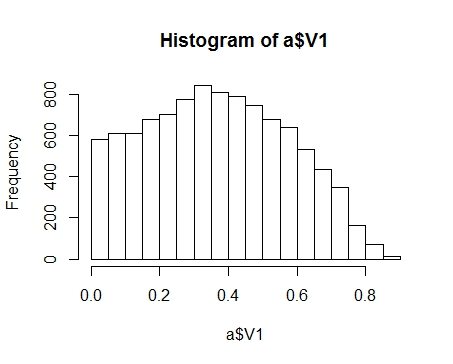
\includegraphics[width=6cm]{img/shrimpHistMATLAB} \\
		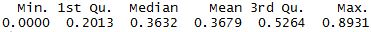
\includegraphics[width=5.5cm]{img/histSummML}
    \begin{center} Histogram from Matlab simulations \end{center}
    \column{.5\textwidth}
    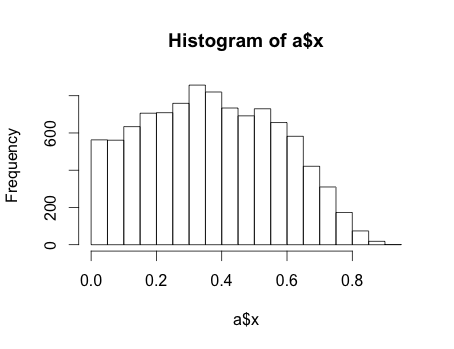
\includegraphics[width=6cm]{img/Rplot} \\
		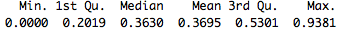
\includegraphics[width=5.5cm]{img/sumAMAN}
    \begin{center} Histogram from C simulations \end{center}
  \end{columns}
\end{frame}



\begin{frame}{Multiplicative Noise}
\begin{center} 
	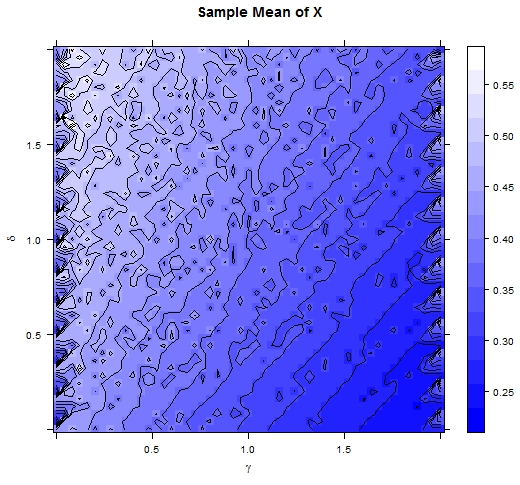
\includegraphics[width=8cm]{img/RplotMultiNoiseContourX} 
\end{center}
\end{frame}

\begin{frame}{Multiplicative Noise}
\begin{center}
	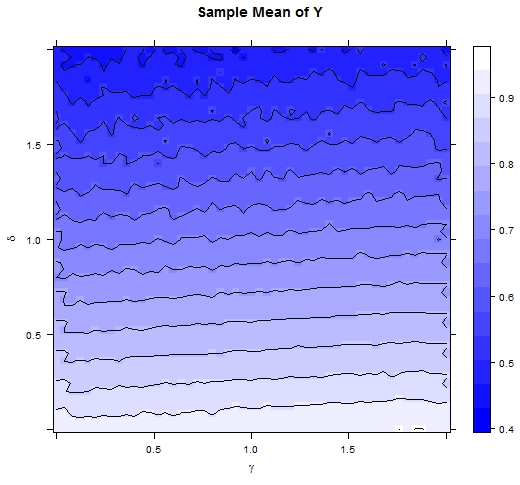
\includegraphics[width=8cm]{img/RplotMultiContourY} 
\end{center}
\end{frame}

\begin{frame}{Multiplicative Noise}
\begin{center}
	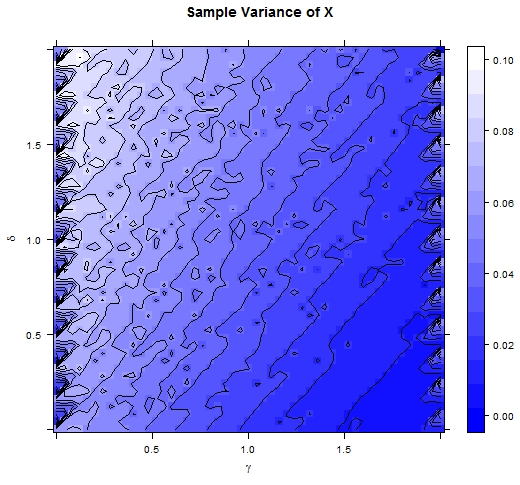
\includegraphics[width=8cm]{img/RplotSampleMultiVarX} 
\end{center}
\end{frame}

\begin{frame}{Multiplicative Noise}
\begin{center}
	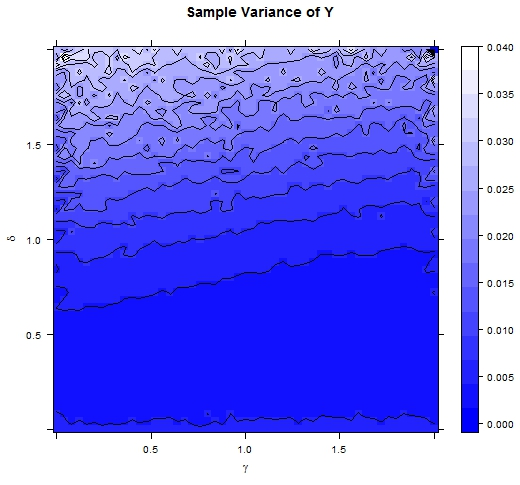
\includegraphics[width=8cm]{img/RplotMultiSampleVarY} 
\end{center}
\end{frame}

\begin{frame}{Additive Noise}
\begin{center}
	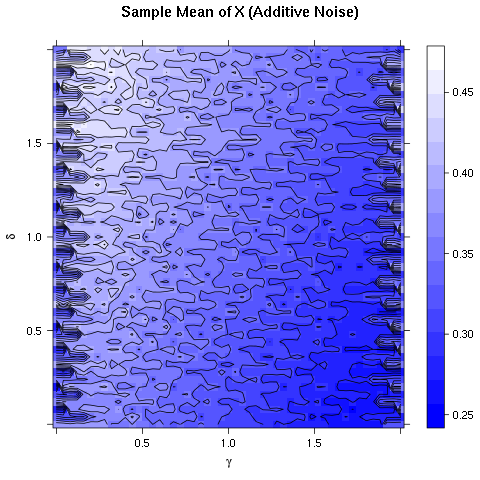
\includegraphics[width=8cm]{img/sampleMeanXAdditiveNoise} 
\end{center}
\end{frame}

\begin{frame}{Additive Noise}
\begin{center}
	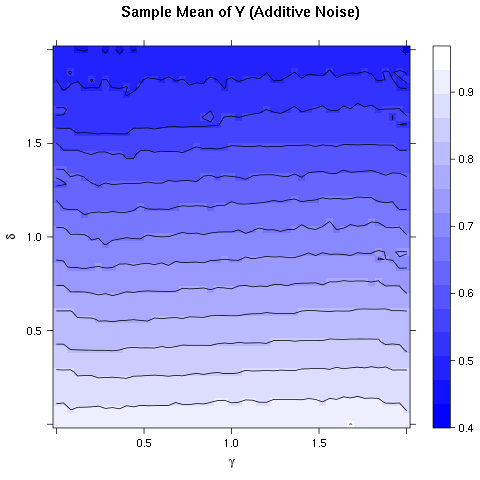
\includegraphics[width=8cm]{img/sampleMeanYAdditiveNoise} 
\end{center}
\end{frame}

\begin{frame}{Additive Noise}
\begin{center}
	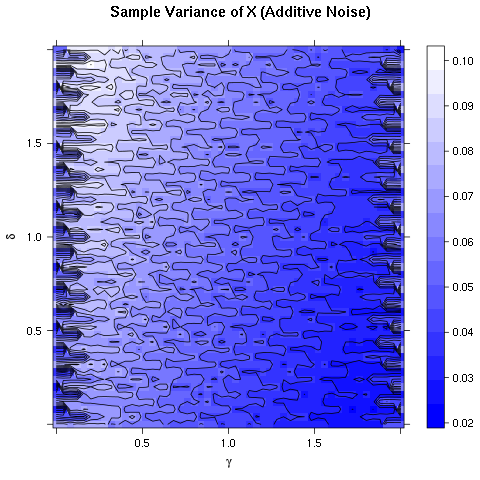
\includegraphics[width=8cm]{img/sampleVarianceXAdditiveNoise} 
\end{center}
\end{frame}

\begin{frame}{Additive Noise}
\begin{center}
	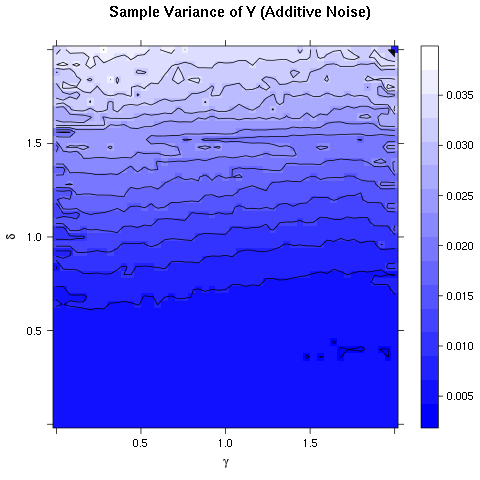
\includegraphics[width=8cm]{img/sampleVarianceYAdditiveNoise} 
\end{center}
\end{frame}

